%!TEX root = ../../Heun_Dale_Haney_A_dynamic_approach_to_input_output_modeling.tex
%%%%%%%%%%%%%%%%%%%%% chapter.tex %%%%%%%%%%%%%%%%%%%%%%%%%%%%%%%%%
%
% sample chapter
%
% Use this file as a template for your own input.
%
%%%%%%%%%%%%%%%%%%%%%%%% Springer-Verlag %%%%%%%%%%%%%%%%%%%%%%%%%%
%\motto{Use the template \emph{chapter.tex} to style the various elements of your chapter content.}
\motto{Where there is no reliable accounting 
and therefore no competent knowledge
of the economic and ecological effects of our lives,
we cannot live lives that are economically
and ecologically responsible. 
It is futile to plead and protest and lobby 
in favor of public ecological responsibility while, 
in virtually every act of our private lives, 
we endorse and support an economic system 
that is by intention, 
and perhaps by necessity, 
ecologically irresponsible.~\emph{\cite[p.~26]{Berry1998}}

\hfill---\emph{Wendell Berry}}


%%%%%%%%%%%%%%%%%%%%%%%%%%%%%%%%%%
%%%%%%%%%% Introduction %%%%%%%%%%
%%%%%%%%%%%%%%%%%%%%%%%%%%%%%%%%%%
\chapter{Introduction}
% Always give a unique label
\label{chap:intro}
% use \chaptermark{}
% to alter or adjust the chapter heading in the running head
\chaptermark{Introduction}
%%%%%%%%%%%%%%%%%%%%%%%%%%%%%%%%%%
%%%%%%%%%%%%%%%%%%%%%%%%%%%%%%%%%%
%%%%%%%%%%%%%%%%%%%%%%%%%%%%%%%%%%


%% \abstract{Each chapter should be preceded by an abstract (10--15 lines long) that summarizes the content. The abstract will appear \textit{online} at \url{www.SpringerLink.com} and be available with unrestricted access. This allows unregistered users to read the abstract as a teaser for the complete chapter. As a general rule the abstracts will not appear in the printed version of your book unless it is the style of your particular book or that of the series to which your book belongs.\newline\indent
%% Please use the 'starred' version of the new Springer \texttt{abstract} command for typesetting the text of the online abstracts (cf. source file of this chapter template \texttt{abstract}) and include them with the source files of your manuscript. Use the plain \texttt{abstract} command if the abstract is also to appear in the printed version of the book.}

%% Use the template \emph{chapter.tex} together with the Springer document class SVMono (monograph-type books) or SVMult (edited books) to style the various elements of your chapter content in the Springer layout.

\abstract*{**** Re-write the abstract. ****
In this chapter we give our motivation for writing this book. 
We outline some of the models and subsequent metaphors 
that have been used to describe the economy---clockwork, 
machine, engine---and suggest a new metaphor---the 
metabolism of an organism.
We give an overview of Leontief Input-Output methods
and their extension to include energy and material inputs
and waste flows out of the economy.
We then propose a new Input-Output analysis method,
fitting to the new metaphor of the metabolic economy;
a dynamic accounting framework that includes accumulation of stocks
within economic sectors.}



This book presents a new approach to national accounting that  
incorporates the accumulation of manufactured capital and use of natural capital
into the economic activities tracked by input-output accounting.
Because input-output accounting is central to 
measures of economic activity and economic impact analysis, \cite{Lawson1997}
we believe
managing our capital \emph{stocks} as well as
measuring the \emph{flows} of economic activity (GDP) are vital to 
manage the energy transformations that are upon us.  

%BRH commented out the following on 6.06.2014
%Economies are in constant flux;
%they respond quickly to changes in human behavior
%and evolve in  
%response to changes in 
%the technological and environmental landscape. 
%Economic evolution often occurs in discrete
%jumps rather then smoothly and consistently. 
%In part, this is due to the capital upon which the
%economy relies.

The manufactured and natural capital in existance at a point in time in an
economy represents the physical infrastructure, natural resources, and
ecosystem services available to satisfy the demands of today's producers and consumers. 
They are a bequest from previous generations.
Power plants, for example,
 as well as the roads and rails that carry inputs to them and the grid that connects
them to the end-user, were built for decades ago. Current users of their services
simply expend what is necessary to maintain them. The amount of 
coal reserves available for power are what previous generations
chose not to use.


The existing manufactured and natural capital therefore represents 
the current 
\emph{wealth} of an economy. However, it also
represents a constaint to economic activity. It
reduces the flexibility of the economy to respond nimbly to change.
The power plant, and the roads, rails, and grid associated with it, were also 
designed decades ago. The decision to use coal, for example, and the choices over 
the type of  technology used to clean the production waste, the plant location, 
and the scale of  operation, were made in the past as well.
And, they were likely made with different ecological information,
 assumptions, and values, in mind. 

Similarly, research and development choices 
made by today's industries will affect the economy for many generations
forward. Those decisions are best made in light of a broad array of relevant data.
Identifying where and to what extent current industries are dependent on 
key categories of capital infrastructure is necessary to understanding the
implications of today's technological decisions. For example, as 
automobile manufacturing shifts towards the production of electric vehicles,
it is necessary to understand the extent to which the robotic assemblies used
to produce electric vehicles are dependent on fossil fuel-intensive production
processes. 

% **** MCD - I feel like we need another statement here ****
% Maybe this one? ****
% We must account for this dynamic nature if we are to
% manage our economies more effectively.
% **** Or maybe this one: 
%Like all real-world systems, 
%economies are messy and chaotic;
%they do not march orderly from one state to the next. To fully understand our economies,
%we must appreciate their dynamic nature.

This book also utilizes a new metaphor for the economy
to more easily incorporate manufactured and natural capital
into economic models.
The prevailing machine metaphor that informs 
 economic imagination and policies has run its course.\cite{Liu2012}
The model presented in this book is informed by a new metaphor for the economy: metabolism.
We believe an organic metaphor, one that acknowledges that 
the economy eats, depletes, and excretes as part of its fundamental processes, will
stimulate creative solutions to navigate the challenging landscape that lays ahead.

It is important to talk explicitly about the metaphor for the economy
as it relates to input-output accounting. 
We use metaphors to simplify and make sense of the world around us.
They influence us as stories we tell ourselves to convey meaning,
to teach ourselves about the world.
Metaphors particularly inform 
the mental and empirical models we construct of the economy.
And, as we collect data
to assess the validity of those models,
our perception of the world is molded and shaped
by our accounting;
the very accounting that was initially informed
by the stories we told ourselves about the economy.
%They tell us what aspects of the world
%are important to value 
%(in the literal sense of making measurements),
%and also, by extension, 
%which parts of the world (literally) have no value.
%This process has a deeper normative consequence: 
%the aspects of the world to which our models ascribe
%value become \emph{valuable},
%and those ascribed no value become \emph{worthless}.


We believe that traditional  models of the economy
based on a machine metaphor ascribe insufficient value 
to important drivers of real economic growth,
including the extant manufactured and natural capital. 
This book illustrates what a metabolic metaphor for 
the economy provides. It highlights manufactured and natural capital stock maintenance
as key activity of the economy. The following 
sections reveal the urgency of including economic-environmental
transactions as part of 
economic activity and the severity of the problems that
have resulted from relying on envisioning the economy as
a perpetual motion machine for too long.


%%%%%%%%%% Limits %%%%%%%%%%
\section{Limits: Extraction, substitution, and assimilation}
\label{sec:limits}
%%%%%%%%%%

As metaphors give rise to models, 
economic models lead to accounting systems that organize data
to affirm or deny model predictions.
National accounts, 
particularly in the US, 
were established to measure the things that 
an economic model based on a machine metaphor values most: 
output. The US system of national accounts measures output (Gross 
Domestic Output) and anything that increases output counts
as an increase in economic growth. In the macroeconomy, \emph{output}
to one sector is \emph{input} to another. National accounting systems easily capture changes in \emph{income}, 
but do not so easily capture changes to the source of a nation's income: its \emph{wealth}.
National accounts do measure investment and depreciation of manufactured capital, but in a very limited way, 
and not in a way that 
allows analysis of the capital dependencies between economic sectors.\cite{Streitwieser:2011aa}

Natural capital is not captured at all in national accounts in the US (although
most other developed countries have some form of accounting for natural capital). 
The US does not even have the ability to track the important categories of materials and energy,\footnote{Note that
	income is counted as a monetary rate (e.g.\ \$/year), 
	not a physical rate (e.g.\ kg of material per year)
	or an energy rate (e.g.\ kJ of energy per year).} 
in a way that can inform meaningful economic discussion or
lead to enlightened natural resource and energy policies.
Whether you think this is a problem depends, in part, on:
whether you think the world's economies are approaching 
	natural resource extraction limits;
whether you think the materials and energy upon which our economies currently depend
	can be easily substituted by other, readily-available, inexpensive resources; and
whether you think that the world's economies have exceeded 
	the biosphere's waste assimilation capacity.


%+++++++++ Natural resource extraction limits ++++++++++
\subsection{Natural resource extraction limits}
\label{sub:natural_resource_extraction_limits}
%+++++++++

For many commodities, 
supply is becoming scarce relative to demand, 
with oil providing, arguably, the most important example. 
Both economic and physical arguments can be used to show that the world is facing
natural resource extraction limits.

Economic theory predicts that as demand for a product increases,
the increased profitability of rising prices 
will induce current producers to increase supply, 
entice new producers to enter the market,
and encourage other producers to offer close substitutes. 
In the case of natural resources, if that does not occur
there is evidence that resource extraction limits are being reached.
This is happening today in the oil market.
For much of the twentieth century, the price of oil remained below \$20 per barrel.
However, in the 2001--2008 timeframe,
the inflation-adjusted price of oil increased 260\%,
from around \$35 to a peak of \$126 per barrel 
(in constant 2010 USD).
During the same period,
world oil production rose from 
78~million barrels per day to 86~million barrels per day,
an increase of only 10\%.\cite{EIA2014}
Since 2010, the price of oil has remained over \$80 per barrel,
suggesting that production cannot increase quickly enough to bring prices
back down to historical levels.
Persistently high prices for such an important commodity
suggest very real limits to production; 
that supply is constrained relative to demand. 
We are reaching natural resource extraction limits.

On a physical basis, 
it is evident that easier-to-reach resources are extracted first. 
After the easier-to-reach resources are depleted (such as oil in West Texas),
more difficult-to-extract resources must be pursued,
further offshore,
in harsher environments, and
with enhanced techniques 
(such as steam flooding or hydraulic fracturing).
Sometimes, new, energy-intensive techniques are required 
for difficult deposits, such as oil sands.
Turning to materials extraction, the production of finer-grade ores
requires the processing of greater amounts of raw material, 
resulting in increasing mining tailings.\footnote{Mining tailings
	are the unwanted materials that remain after mining processes
	have removed economically valuable materials.\cite{Mudd2007}
	}
The processing of extra raw material takes more energy, and 
the energetic cost of extracting many materials is certainly increasing.\cite{Hall1986, Mudd2010, Hall2011}
This process has been labeled the ``Red Queen'' effect, 
where we must extract increasingly more resources to achieve the same
level of production---run faster and faster just to stay in 
the same place.\cite{Lees1975, Ross1988, Murray2013, Murphy2014}
The facts that (a) producers continue to reach deeper and farther 
and (b) energetic costs of production continue to rise
are further evidence that the world is reaching natural resource extraction limits.


%+++++++++ Substituion ++++++++++
\subsection{Substitutability of natural resources}
%+++++++++

The ability to substitute human-made capital for natural resources
or one natural resource for another 
may alleviate the problem of natural resource scarcity relative to demand,
at least temporarily.
There are many historical examples of this sort of substitution occurring,
particularly in the energy sector.
Deforestation within Europe,
primarily for fuel to smelt iron,~\cite{Smil1994}
prompted the switch from wood to coal.
Whale oil was replaced by petroleum-based kerosene for lighting and
coal has also been replaced by oil for other uses, 
especially transportation.\cite{Weissenbacher2009}
More recently, natural gas has begun to replace oil in many applications.
Therefore, goes the argument, 
substitution may continually stave off resource scarcity.
But, there is evidence both at the macroeconomic level and 
at a technical level that there are limits to energy substitution.

Pelli, in a study of 21 countries 
found that clean\footnote{Nuclear, 
	conventional hydroelectric power, wood and waste biomass, 
	geothermal, solar/photovoltaic, and wind
	}
and dirty\footnote{Coal, 
	petroleum, natural gas, and other gasses
	}
inputs to electricity production
are complementary (as opposed to substitutable).\cite{Pelli:2012wv}
His conclusion is dire:

\begin{quote}
	On the one hand, according to the model, 
	if we keep producing electricity using dirty inputs, 
	we head toward an environmental disaster. 
	On the other hand, looking at the empirical results, 
	it seems impossible to stop producing electricity with polluting resources. 
	The policy implication of this paper thus, 
	seems to be that we need more important subsidies to research, 
	as fast as possible, 
	and high carbon taxes combined with a complete halt 
	of the growth rate of the production of electricity. 
	In this way, according to the model, 
	we may be able to avoid an environmental disaster.\cite[p.~25]{Pelli:2012wv}
\end{quote}

In a meta-analysis of 15 papers that studied 
the economic evidence for macro-substitutability
among factors of production (materials, capital, labor, and energy), 
de Wit et.\ al.~\cite{de-Wit:2013aa} found that the elasticity of substitution was 
below unity for all combinations of factors of production.
Furthermore, they argue that, 

\begin{quote}
	[because all of the] results show elasticity of substitution below unity, 
	none of the factor inputs are perfectly substitutable and 
	all tend toward complementarity in varying degrees. 
	Such results suggest that transitions 
	from one production or consumption structure to another 
	can be disruptive and that the transitions 
	need to be modeled dynamically to the extent possible.\cite[p.~8]{de-Wit:2013aa}
\end{quote}

There are limits to substitution from a technical point of view, as well.
For example, there are no known substitutes for oil 
in many sectors of the economy.\cite{Hirsch2005}
Biofuels were hailed by many as a viable alternative to fossil fuels, but
there is not enough land for biofuels to meet current liquid fuel demand
without displacing food production.
These realities highlight the fact that within tightly coupled, 
complex systems (such as the energy--food system), %chktex 8
changes in one part of the system often have unintended consequences elsewhere.
For example, 
the US obtains 13 billion gallons of bio-ethanol 
(less than 10\% of the 134 billion gallons of domestic fuel consumption in 2012)
by diverting approximately 40\%
of domestic corn production for biofuel.\cite{EIA2014, USDA2014}
This policy has had dramatic impacts on global food security,
with each billion gallon increase of biofuel production believed to cause
a 2--3\% increase in corn prices.\cite{Kemick2013} 
%**** Mik, \$2--3 increase PER WHAT? MKH ****
%**** MCD - \$2--3 increase in corn price per billion gallon increase in ethanol production.
%Would you prefer to have it that way round? ****
%**** MCD - sorry my bad, it was 2-3% ****

Often, the substitution of manufactured resources for natural resources
requires the use of greater amounts of energy.
For example, the production of fresh water from recycled or seawater
can be particularly energy intensive.
Thus, the substitution of a manufactured resource (desalinated water)
for a natural resource (fresh water)
requires greater inputs of natural resources (in this case, free energy) to achieve.
Whereas material resources can, at least in theory,
be recycled indefinitely,
free energy is the ultimate limiting resource, 
because energy cannot be 100\% recycled.

For many commodities today, limited or negligible substitution is possible,
and the complex, highly-coupled nature of modern economies
often leads to unintended consequences (usually involving increased energy consumption)
when substitution is technically possible.
We are reaching limits of substitutability for many important 
materials and energy sources for our 
economies.\footnote{The issues of resource scarcity and substitution
	will be revisited in 
	the Materials chapter~(\ref{chap:materials}) and
	the Energy chapter~(\ref{chap:direct_energy}).}


%+++++++++ Overloading assimilative capacity ++++++++++
\subsection{Overloading the biosphere's assimilative capacity}
%+++++++++

%**** Mik: I've taken a 3rd (4th?) run at this. 
%What do you think now? MKH ****

There are many examples of society locally exceeding 
the assimilation capacity of the biosphere.
In 1952, London city experienced a lethal smog cloud,
due to coal-burning power stations,
that, according to some, 
claimed as many as 12,000 lives.\cite{Davis2002,Bell2004}
Many Chinese cities are currently experiencing similar problems.
Such point-source, localized environmental problems can often be overcome
by regulations.
In Britain, two Clean Air Acts regulated emissions from both
industrial and domestic sources.\cite{Brimblecombe2006}	
In the US, emissions regulations in California have 
significantly reduced Los Angeles' legendary smog problem.

However, there is mounting evidence that systemic ecosystem
damage occurs due to the externalized costs
of growing economies.
Of course, the perspective of \emph{external} and \emph{internal} is subjective.
A cost externalized by one agent
must be internalized by another.\cite{MEA2005,Ewing2008}
So, natural systems often bear the burden of human production.
So-called ``free'' natural resources are exploited,
land-use is altered to better suit society's needs,
and other species are marginalized by the encroachment of human activity.\cite{schnaiberg1980}
In many cases, as more waste is deposited into ecosystems,
and as the structures of ecosystems are permanently altered for human desires,
the assimilation capacity of the biosphere declines.
When the assimilation capacity of the biosphere is exceeded, 
services provided by the biosphere may be disrupted.\cite{UNMEA2005}

Many wastes are either emitted from multiple locations or have 
significant non-local effects. 
Examples include:
algal blooms and so-called ``dead zones'' due to over-use of agricultural fertilizers;
over-use of agricultural pesticides;
build-up of persistent organic pollutants, especially endocrine disruptors, such as PCBs 
	and BPAs;\footnote{Polychlorinated biphenyl (PCB) 
		is a synthetic organic chemical often used as 
		a dielectric or coolant in electrical equipment.
		It is a known carcinogen.
		Bisphenol (BP) A is a carbon-based synthetic compound used in the production
		of plastics and epoxy resins. It exhibits hormone-like properties at high doses.
		}
bio-accumulation of heavy metals released due to mineral extraction and industrial processing;
ozone depletion due to release of chlorinated gases (primarily halocarbons);
acid rain due to release of sulfur dioxides;
release of radioactive materials;
detergents in sewage;
invasive species;
oil spills;
and, of course, greenhouse gas emissions.\cite{UNMEA2005, Butler1978, Walker2012}
In each case, human economic activity has increased the concentration
of wastes to the point where the biosphere can no longer maintain 
previous levels of ecosystem service.
We are reaching assimilation limits.


%+++++++++ Material and energy transformation ++++++++++
\section{Material and energy transformation}
%+++++++++

Because the world is facing natural resource extraction limits
(especially for some forms of energy)
and because we are exceeding the assimilative capacity of the biosphere,
it follows that a structural transformation of the economy is imminent.
Society cannot accelerate rates of material extraction
and waste production indefinitely.

Because substitutability is finite, 
it follows that reaching the extraction and assimilation limits 
of the biosphere will bring significant societal challenges.
The question is: how will this transformation unfold?
How will our economies cope with the challenges?

We contend that materials and energy transformations will either  
\emph{happen to} us, or we will \emph{plan for} them.
At present,
transitions are happening \emph{to} us:
very little materials or energy planning occurs
at the industry-wide or government level.\footnote{On the world stage, 
	notable exceptions include the UN Environment Programme's 
	International Resource Panel~\cite{UNEP-IRP:aa}
	and the United Nations System of Environmental-Economic Accounting.\cite{UNSEEAWeb}
	}
Because it is likely that unplanned transformations will be rocky and difficult,
we believe that some type of planning is needed.

Clearly, the first step for effective planning 
is knowledge of the current state of affairs.
We need to know the existing materials and energy structure of our economies. 
This implies that we should know the rates at which 
the world's economies consume raw materials and emit wastes back to the biosphere.
We need to understand the connections between the biosphere and the economies of the world.
But, we also need to know how materials and energy consumption 
are likely to evolve in the future.
We should know where and at what rate 
materials and embodied energy accumulate 
in economic infrastructure. 
We should know the material and energy costs of maintaining the
increasingly-complex infrastructure of society.
We should have a sense of the transient and variable nature of economies
and the materials and energy flows that sustain them.
In short, we need to be \emph{accounting for the environment}!\footnote{The title 
	of this book is a \emph{triple entendre}.
	First, we should take the environment ``into \emph{account}''
		when developing our system of national accounts.
		As discussed in the Preface, at present, we are not.
	Second, we should be maintaining and disseminating
		records or accounts of environmental assets. 
		In this usage, \emph{account} is a noun
		referring to our endowment of natural resources.
	Third, we should develop our system of national accounts 
		\emph{for the benefit of} the environment, 
		with the understanding 
		that a healthy environment sustains a healthy economy.
		In this sense, \emph{accounting} is used as a verb with a telos.
}
Despite this need, we (i.e., society at large) 
are not accounting in a way that helps us plan 
for the economic challenges that will accompany 
the impending materials and energy transformation.
All of which leads to a burning question,
one with significant consequences for the future:

\begin{quote}
{\normalsize{How can you maintain a system of national accounts without 
accounting for natural assets?}}
\end{quote}

\noindent{}With that in mind, the purpose of this book is to 
develop a dynamic model to help us
``account for the environment''
with the objective of planning for impending materials and energy transformations.

%%%%%%%%%% Metaphors and Models %%%%%%%%%%
\section{Metaphors and models}
\label{sec:metaphors_and_models}
%%%%%%%%%%

Before moving ahead with the work of developing our dynamic model,
it is useful to consider how society has come to this point.
How is it that we don't account for the environment when 
considering materials and energy flows into, within, and out of the economy?
The classical economists certainly appreciated the dependence of
economic activity on bio-physical processes.\cite{Cleveland1987, Hall2011, Dale2012}
However, somewhere between William Stanley Jevons' 1865
assessment that
``the very existence of Britain, as a great nation''~\cite[IV.3]{Jevons1865}
was tied to a continued supply of low-cost coal 
and Julian Simon's 1998 statement that
``natural resources are not finite in any economic sense,''~\cite[p.~54]{Simon1998} %chktex 38
the importance of the biosphere was lost.

%*** BRH isn't this quote supposed to indicate that running out of coal from over production
%and the recursive need for coal to produce more coal
%was threatening GB? That quote doesn't seem to make that very clear ***
%**** MCD - no, I simply wanted a statement from an eminent economist on the importance of natural resources.
%It doesn't have to be from Jevons and I'm certainly open to a different quote ****
%**** Matt says: The entire paragraph from Jevons (\url{http://www.econlib.org/library/YPDBooks/Jevons/jvnCQ4.html}) is
%\begin{quote}
%	Now, in coal-mining, we must discriminate the physical and commercial possibility. 
%	The second presupposes the first, but does not follow from it. 
%	The question is a twofold one:
%	Firstly, is it physically possible to drive our coal-mines 
%	to the depth of 4,000, 5,000, or 6,000 feet? 
%	and, secondly, is it commercially possible when 
%	in other parts of the world coal is yet being worked in the light of day? 
%	The very existence of Britain, as a great nation, is bound up in these questions.
%\end{quote}
%It doesn't seem like it was coal production, per-se that Jevons was tying
%to Britain's greatness.
%Rather, it was \emph{continued} coal production and the ability to mine deeper
%at low cost that was tied to Britain's greatness.
%
%Perhaps the sentence can be modified to say:
%However, somewhere between William Stanley Jevons' 1865
%assessment that
%``the very existence of Britain, as a great nation''~\cite[IV.3]{Jevons1865}
%was tied to continued low-cost coal production% from deepening mines
%and Julian Simon's 1998 statement that
%``natural resources are not finite in any economic sense,''~\cite[p.~54]{Simon1998} %chktex 38
%the importance of the biosphere was lost.



%+++++++++ The clockwork metaphor ++++++++++
\subsection{The clockwork metaphor}
\label{sec:clockwork_metaphor}
%+++++++++

Indeed, most economics textbooks today depict the economy 
as in Figure~\ref{fig:perp_motion_1}.
Goods and services flow from the production sector
to the household sector~(consumption)
in exchange for payments.
The factors of production (labor and capital)
flow from the household sector to the
production sector in exchange for wages and rents.
Attention is primarily focused on the circular flow
of money~(dashed line).


\begin{figure}[!ht]
\centering\
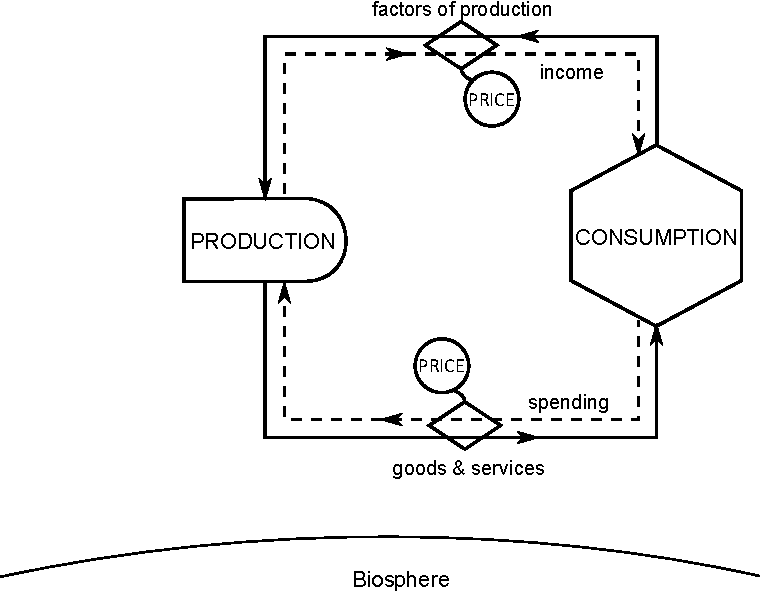
\includegraphics[width=\linewidth]{Part_0/Chapter_Introduction/images/Perpetual_motion_1.pdf}
\caption[The traditional model]{In the traditional model, the economy 
is represented as a circular flow of goods and services between two sectors. 
The producers manufacture goods and services 
by taking in labor and capital. 
Consumers exchange labor for wages 
which are used to purchase 
the goods and services of the producers.}
\label{fig:perp_motion_1}
\end{figure}

This traditional model of the economy~(Figure~\ref{fig:perp_motion_1}) 
is unashamedly mechanistic.
General equilibrium models of the economy
~\cite{Walras1892, Walras1993}
were borrowed directly from classical physics' models of 
mechanical equilibrium which, in turn, arose from the 
``clockwork universe'' metaphor.\cite{Ingrao1990}
As discussed above, 
the clockwork metaphor is an example  
of a simplification that helps us make sense of the world around us.
Metaphors inform our thinking about the real world,
but consequently,
they also constrain our ability to frame reality.
We mistake the model-metaphor for reality, and
we interact with reality in the same manner 
as we interact with the abstract objects of our
models.\footnote{This fallacious process is called
	\emph{reification}; the making (\emph{facere}, Latin) real of
	something (\emph{res}, Latin) that is merely an idea.
	Alfred Whitehead refers to this as
	\emph{the fallacy of misplaced concreteness}.\cite{Whitehead2011}
	}
Classical physics told us the universe is
\emph{like} clockwork, 
so we began to interact with the universe
as if it \emph{really were} clockwork.
It then became easy to collect data that confirmed the clockwork model,
because the model told us which data to collect.

The clockwork metaphor and the traditional model of the economy
preclude any sort of connection 
between the economy and the biosphere.
Thus, only the internal dynamics of the economy are important. 
They tell us that natural resources are unimportant, 
effectively assuming that the biosphere will always provide.
If a particular resource becomes scarce, 
substitution to a different, more-readily-available resource will be made.
They tell us that wastes are quantitatively unimportant, 
effectively assuming that the biosphere has infinite assimilative capacity.
Finally, the clockwork metaphor and traditional model of the economy 
tell us that economic forces 
(through prices and the market mechanism) 
are sufficient to efficiently guide any necessary transition
within the economy.
Any physical constraints that the biosphere places on 
the allocation of resources, distribution of outputs, and 
scale of an economy 
are outside the scope of neoclassical economic discussion.\cite{Daly1995}
%``Natural resources are not finite in any economic sense.''~\cite[p.~54]{Simon1998} %chktex 38
In short, the clockwork metaphor and the traditional model of the economy 
tell us that the clockwork-economy can and will carry on.

Because Figure~\ref{fig:perp_motion_1} has no flow of energy
into the economy,
we may consider it a perpetual motion machine
of the \emph{first kind}:
the economy works without the input of energy, thus violating
the First Law of Thermodynamics---the 
law of conservation of energy.\cite{Rao2004}
However, thermodynamics tells us that all physical processes 
require a transfer of energy.


%%%%%%%%%% Resource metaphors %%%%%%%%%%
\subsection{The machine metaphor}
\label{sec:machine_metaphor}
%%%%%%%%%% 

%The real circulatory system is connected to the lungs,
%from where it takes in oxygen,
%and to the digestive system, 
%where it takes in processed food,
%which are passed to the cells throughout the body.
%This is a major function of the blood:
%to act as an intermediary between the input of energy
%and material resources,
%the food we eat and air we breathe,
%and the internal working of the body.
%The circulatory system is necessarily connected 
%to its environment and circulates energy and materials
%that have been extracted from it.


%Current economic models assume
%continued economic growth is possible, 
%necessary, and good. Thus, questions about
%the appropriate scale for the economy 
%are not asked. Even if they were, those questions
%could not be answered because the
%required data are not collected. 
%As the population of the world grows, will we 
%be able to create enough cars to satisfy the growing demand?
%Can we meet the increasing demand for steel, rubber, glass,
%and fuel without considering the consequences? 
%Will there be enough energy to power the 
%automobile factories as 
%well as the increasing number of cars? Will the 
%environment be able to assimilate an ever-increasing 
%amount of pollution?
%
%The mainstream response to those questions
%has been to assume that over a long enough
%time period, economies are not bound by physical 
%limits because of \emph{factor substitutability}.
%A particular energy resource (oil) may be in short supply,
%but our technological expertise---which expands
%as the economy grows---will allow us to substitute
%another resource (coal) for it.
%Substitution may continue indefinitely thus, so
%goes the story,
%the only limiting resource is
%human ingenuity.\cite{Simon1981, Simon1998}
%
%This assumption was thrown into stark relief following the oil
%shocks of the Seventies.
%Suddenly the global economy was thrown
%into reverse for lack of one fundamental resource.
%The necessity of including,
%at the very least,
%energy resources into the economic picture
%spurred the efforts of early (net) energy 
%analysts.\cite{Gilliland1975, Chapman1976}


The limits of the clockwork metaphor and traditional model of the economy were 
exposed by the oil shocks of the 1970s.
Suddenly the global economy
``stalled'' due to lack of 
% was thrown into reverse by 
a single, highly-constrained resource:
fuel.
Many came to realize that energy input is required
for successful operation of an economic ``engine.''
Thus, a machine metaphor and 
accompanying engine model for the economy 
rose to prominence
in the late 1970s and early 1980s.
The need to include energy resources
in the economic picture
spurred the efforts of early (net) energy 
analysts.\cite{Gilliland1975, Chapman1976}

The engine model accounts for energy flows from the biosphere 
to the economy and is shown in Figure~\ref{fig:perp_motion_2}.
With the new metaphor, the economy changed from 
an \emph{isolated} system~(Figure~\ref{fig:perp_motion_1}) to 
a \emph{closed} system~(Figure~\ref{fig:perp_motion_2}). 
The importance of input energy is acknowledged, 
but wastes are absent.
And, the biosphere is relegated to the position
of provider of energy resources;
the gas station of the economy.\cite{Norgaard2010}

\begin{figure}[H]
\centering\
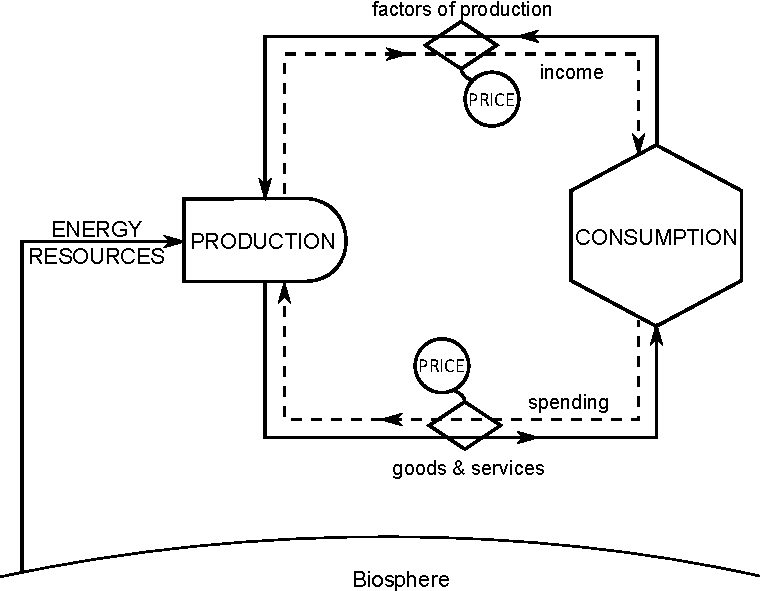
\includegraphics[width=\linewidth]{Part_0/Chapter_Introduction/images/Perpetual_motion_2.pdf}
\caption[The machine model]{The machine model of the economy includes
flows of energy into the economy from the biosphere.
This may be considered a perpetual motion machine 
of the second kind.}
\label{fig:perp_motion_2}
\end{figure}

The machine metaphor and engine model are still very much mechanistic.
Much like the engines of the Industrial Revolution,
the economic engine is assumed to be well-behaved and amenable to control.
Even today, machine metaphors abound in our economic discussions.
We speak of ``fueling'' the ``economic engine'' 
lest it should ``stall.''~\cite{Liu2012}
Like a well-running engine, the economy is assumed 
to be resilient to small or even quite large perturbations.  
It can either self-correct, 
or be corrected with adjustments to
a few predictable policy levers.

But, in light of the challenges discussed above,
how accurate is the engine model?

According to the Second Law of Thermodynamics,
all real-world processes involve the degradation
of material and especially energy resources
and the creation of entropy.
High quality (low entropy) material and energy come in;
low quality (high entropy) material and energy go out.
The depiction in Figure~\ref{fig:perp_motion_2} 
can be classified as a perpetual motion machine
of the \emph{second kind}:
it perfectly converts energy resources into 
work~(useful services) without generating
any entropy,
in violation of the Second Law of Thermodynamics.
Because the generation of high entropy~(low quality)
output is a \emph{necessary} feature of \emph{all} processes 
(including economic processes)
then the generation of wastes is a \emph{normal} feature of
economic processes,
not an anomaly.
Within a closed system, such as the earth,
these wastes soon accumulate,
necessitating the change to a ``spaceship'' economy,
wherein account is made of the waste outflows from
the economy.

We need a different model.


%%%%%%%%%% A new metaphor %%%%%%%%%%
\subsection{A new metaphor}
\label{sec:new_metaphor}
%%%%%%%%%% 

When our collective imagination is stuck on a metaphor that 
informs models in which the economy is isolated from or closed to the biosphere,
the suggestion to ``account for the environment'' is unconvincing, and 
the challenges cited earlier (natural resource extraction limits,
difficulty of material and energy substitutions, and 
exceeding the biosphere's waste assimilation capacity)
seem unimportant. 

Mounting evidence shows otherwise.

Thus, we need to find a new way to understand the complex, 
messy dynamics of real-world economies;
we need a new way to make sense of real-world events;
we need a new way to learn where and how economies can go wrong; and
we need to plan for the impending materials and energy transformations.
To do so, we had better be counting data to assess \emph{dynamic} models
guided by metaphors that tell us \emph{more} than ``the world is an orderly place.''
Our counting needs to be informed by metaphors and models that are
able to cope with rapid transience and transformation,
not just ordered stability.

We need a new metaphor.


%%%%%%%%%% An Apt Metaphor %%%%%%%%%%
\section{An apt metaphor for the economy}
\label{sec:apt_metaphor}
%%%%%%%%%%

If the clockwork and machine metaphors are unsuitable, 
what might an apt metaphor for the economy be?
And, if we find an apt metaphor, what types of models would it inform?
Furthermore, what data would the models tell us to collect?
That is, how should we go about accounting for the environment?
From here to Section~\ref{sec:our_new_model}, we answer the above questions
and, in the process, sketch the outline of our new approach 
to thinking about and accounting for materials, energy, and the economy.
Later chapters will flesh out this sketch.

To begin the search for an apt metaphor, 
we might first ask the question, 
what characteristics should the metaphor possess?
In our opinion, an apt metaphor should account for the facts 
that a real economy:

\begin{enumerate}
	\item{\label{itm:intake}intakes material and energy from the biosphere}
	\item{\label{itm:internal_exchange}exchanges materials, energy, and information internally}
	\item{\label{itm:discharge}discharges material and energy wastes to the biosphere}
	\item{\label{itm:energetic_costs}is affected by energetic costs}
	\item{\label{itm:scarcity}is affected non-linearly by scarcity 
			in the face of low substitutibility}
	\item{\label{itm:non-linear}can change non-linearly or in discrete steps with the potential 
			for structural transformation}
	\item{\label{itm:embodies}embodies energy in material stocks, and}
	\item{\label{itm:robust}maintains organizational structure despite changes 
			in the environment.\footnote{We note that 
				several areas of the literature speak to the items in this list.
				Material Flow Analysis~(MFA) and 
				Economy-Wide Material Flow Analys~(EW-MFA)
				stress the importance of
				material intake by the economy. 
				(See Section~\ref{sec:materials_auto}.)
				The Input-Output~(I-O) method highlights the effects of internal exchanges
				of material and information with economies. 
				(See Chapter~\ref{chap:intensity}.)
				Life-Cycle Assessment~(LCA) techniques focus attention 
				on otherwise-neglected wastes. 
				(See Section~\ref{sec:intensity_auto}.)
				Net Energy Analysis~(NEA) predicts that energy resource 
				scarcity reduces Energy Return on Investment~(EROI)
				and increases energy prices.
				(See Sections~\ref{sec:B_energy} 
				and~\ref{sec:resource_quality_and_irreversibility}.)
				The Energy Input-Output~(EI-O) method gives prominence to energetic costs
				for internal material and energy flows.
				(See Chapter~\ref{chap:intensity}.)
				And, thermodynamic control-volume modeling describes
				transient behavior and system transformations.
				(See Chapters~\ref{chap:materials}--\ref{chap:value}.)
			}}
\end{enumerate}

Living metabolisms\footnote{The 
	Greek root of metabolism 
	(\emph{metabol$\bar{e}$}) means ``change.''}
exhibit the characteristics in the list above.
Metabolisms and the organisms they support
are intimately connected with the biosphere:
they withdraw materials and energy from the biosphere~(\ref{itm:intake}), 
transfer materials and energy internally via metabolic processes~(\ref{itm:internal_exchange}),
and discharge wastes back to the biosphere~(\ref{itm:discharge});
in fact, their very survival depends on these processes.
Extending Figures~\ref{fig:perp_motion_1} and~\ref{fig:perp_motion_2}
to include the facts in items~(\ref{itm:intake})--(\ref{itm:discharge}), % chktex 36
we obtain Figure~\ref{fig:metabolic_economy}.
Metabolisms are affected by energetic costs~(\ref{itm:energetic_costs}): 
an organism that obtains less energy than it expends is doomed.
Withholding life-sustaining resources brings drastic, non-linear
consequences for any metabolism~(\ref{itm:scarcity}).
Metabolisms enable non-linear, structural transformations
in their host organisms (e.g., metamorphosis, puberty, and evolution)~(\ref{itm:non-linear}).
And, energy absorbed into a metabolism is considered to be ``embodied''
in the cells of the organism~(\ref{itm:embodies}).
Metabolisms exist in a state of dynamic stability~(\ref{itm:robust}),
adjusting and readjusting to maintain their internal conditions
despite changes in the environment;
for a metabolism, equilibrium means death!

The economy is society's metabolism.\cite{F-K1998, Giampietro2000, Giampietro2013}

\begin{figure}[!ht]
\centering\
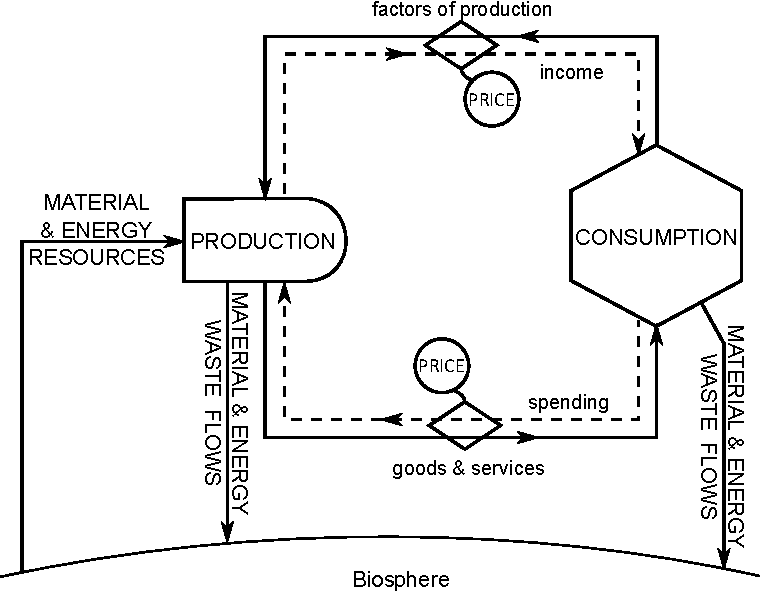
\includegraphics[width=\linewidth]{Part_0/Chapter_Introduction/images/PERKS.pdf}
\caption[The metabolism model]{The metabolism model provides a comprehensive view 
of the economy, fully consistent with the laws of thermodynamics, 
including degraded resources (waste) expelled 
to the environment as a necessary consequence of economic activity.}
\label{fig:metabolic_economy}
\end{figure}


%%%%%%%%%% Apt Models %%%%%%%%%%
\section{An apt material, energy, and economy model}
\label{sec:apt_models}
%%%%%%%%%%

As discussed in Section~\ref{sec:metaphors_and_models}, 
metaphors give rise to models.
So, a natural question is: 
``what types of models does the metabolism metaphor inform?''

In our opinion, apt models should have the following characteristics:

\begin{enumerate}
	\item{\label{itm:flows}account for flows of materials and energy 
			into, within, and out of the economy,}
	\item{\label{itm:accumulation}account for accumulation of materials and energy 
			within the economy,}
	\item{\label{itm:metrics}provide metrics that relate energy demands and economic value, and}
	\item{\label{itm:accounting}provide results that are comparable against existing 
			(or expanded) national accounting.}
\end{enumerate}

Material and energy flow balance equations, 
often employed by thermodynamicists, 
can account for both flows~(\ref{itm:flows}) and accumulation~(\ref{itm:accumulation}) 
of materials and energy within systems.
We will adapt an existing Input-Output~(I-O)
energy analysis method to develop a 
technique for obtaining metrics 
of energy and economic value~(\ref{itm:metrics}).\footnote{See Chapter~\ref{chap:intensity}
for details of the I-O method.}
Finally, we note that systems of national accounts use the economic sector
as their level of analysis. 
Thus, apt models should be also implemented at the economic sector level
so that model results can be 
compared against existing (or expanded) national accounting~(\ref{itm:accounting}).


%%%%%%%%%% Our new model %%%%%%%%%%
\section{Our new model}
\label{sec:our_new_model}
%%%%%%%%%%

%**** Add a discussion of the "system" and "boundaries". Discuss levels of disaggregation as a proxy for area of interest ****
%
%**** Emphasize the greater understanding that comes from explicitly modeling accumulation of (embodied) energy and materials within the economy. ****
%
%**** You have to draw boundaries somewhere.****
%
%**** We disaggregate the economy, because that the is the locus of our interest. An ecologist, in contrast, may choose to disaggregated the biosphere to answer questions such as biodiversity, etc. The biosphere is a container with which our system of interest is interacting. Why? An area of interest is the impact of energy transitions on the economy. ****

We contend that society is not accounting materials and energy adequately 
to prepare for the coming material and energy transformations 
**** MCD - metamorphosis? ****.
In Sections~\ref{sec:apt_metaphor} and~\ref{sec:apt_models} above,
we identified a metabolism as an apt metaphor and model for the economy 
to assist the process of developing the knowledge and analysis approaches
necessary to plan for the upcoming transitions.
Some elements of our approach are not new.
We're not the first to claim that a metabolism is an apt metaphor for the economy
(Section~\ref{sec:apt_metaphor}).~\cite{Barradas1936, F-K1998, Giampietro2000, Haberl2001, Daniels2001}
Nor are we the first to claim that an apt model for the economy 
involves material and energy flow equations 
applied at the level of economic sectors using an Input-Output framework.~\cite{G-R1975 ,G-R1979a, Lenzen1998, Hendrickson2006}

But, we are the first to comprehensively include accumulation
of materials and embodied energy in an accounting framework
based on existing systems of national accounts.
We contend that accounting for accumulation 
of materials and embodied energy in economic sectors is essential
for several reasons:

**** Mik, can you have a look at this list? Matt ****

\begin{itemize}
	\item{real economies convert raw materials extracted from the biosphere
		 	into engineered objects that accumulate,  
			embodied as the infrastructure of the economy;}
	\item{accumulated materials and infrastructure require further material and energy flows
			for their operation and maintenance,
			thereby placing additional material and energy demands on the biosphere;}
	\item{accumulated materials and infrastructure depreciate and need to be replaced,
		 	leading to additional material and energy demands on the biosphere,}
	\item{rapidly growing economies have large accumulation rates, 
			and accounting only for non-accumulating,
			consumptive (through-put) flows of material and energy 
			underestimates the energy demands of those economies.}
\end{itemize}

To include this accumulation of materials and embodied energy, 
we had to re-think the I-O framework starting from fundamental assumptions
and then re-derive the I-O accounting equations
to allow for accumulation, as shown in the following chapters. 
Thus, to our knowledge, we are the first 
to systematically derive the I-O equations to account for accumulation
in a thermodynamically-consistent manner.

To complete the outline and scope for our new model, 
the following subsections address
questions of system boundary and what must be counted.


%%%%%%%%%% System boundary %%%%%%%%%%
\subsection{System boundary}
\label{sec:system_boundary}
%%%%%%%%%% 

In Figure~\ref{fig:biosphere_economy},
the economy is shown as embedded within the surrounding environment,
the biosphere.
Materials and energy (yellow arrows) flow around the biosphere,
many of which do not interact with the economy.
Some of the flows are extracted from the biosphere for human purposes.
These flow around (and accumulate within) the economy,
before ultimately being emitted back into the biosphere as waste.
Processes within the biosphere are then able to regenerate some of these
flows making them available again for human use,
for example the conversion of carbon dioxide into oxygen by photosynthesis.

We have chosen to draw the system boundary of this new model around the economy
and focus only on those flows that pass through the economy.\footnote{An ecologist
	is likely have a different focus 
	and study material and energy flows that never enter the economy.
	}
This is the same system boundary used by the
systems of national accounts (SNA),
although the types of flows accounted are different.
As will be seen in later chapters,
the economy (as our main locus of interest) is further disaggregated 
to the level of industrial sectors.
Our primary interest in doing this is that it is important 
to know where materials and energy accumulate in understanding
the structure of our economies.
This will provide us a better model of the economy and
enable greater understanding of the structural transformation that lies ahead.

The biosphere is included in the model, but only at an aggregated level;
it is the container for the economy. 
We ignore material and energy flows that occur only within the biosphere,
but do not enter the economy.
This means that many important issues lie outside the scope of our new model. 
For example, questions of species loss and
bio-diversity remain outside of this system. 

**** MCD - WHICH VERSION OF THE FIGURE DO WE PREFER?? ****


\begin{figure}[!ht]
\centering\
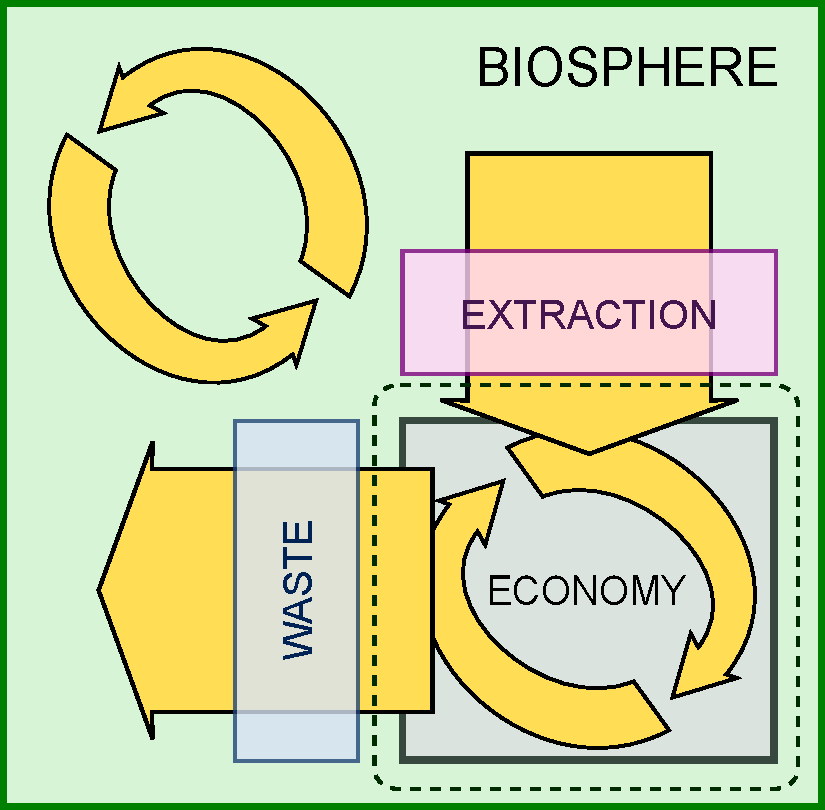
\includegraphics[width=\linewidth]{Part_0/Chapter_Introduction/images/Biosphere_economy.pdf}
\caption[The biosphere and the economy **** MCD - NEED A BETTER FIGURE TITLE ****]
				{The interaction of the economy with the biosphere.
				Materials and energy (yellow arrows) flow around the biosphere.
				Some flows are extracted for human use and enter the economy.
				The materials and energy flow around the economy 
				(as well as accumulating in capital stocks)
				before being emitted as wastes back into the biosphere.
				The size of the arrows does not indicate magnitude of flows.}
\label{fig:biosphere_economy}
\end{figure}

\begin{figure}[!ht]
\centering\
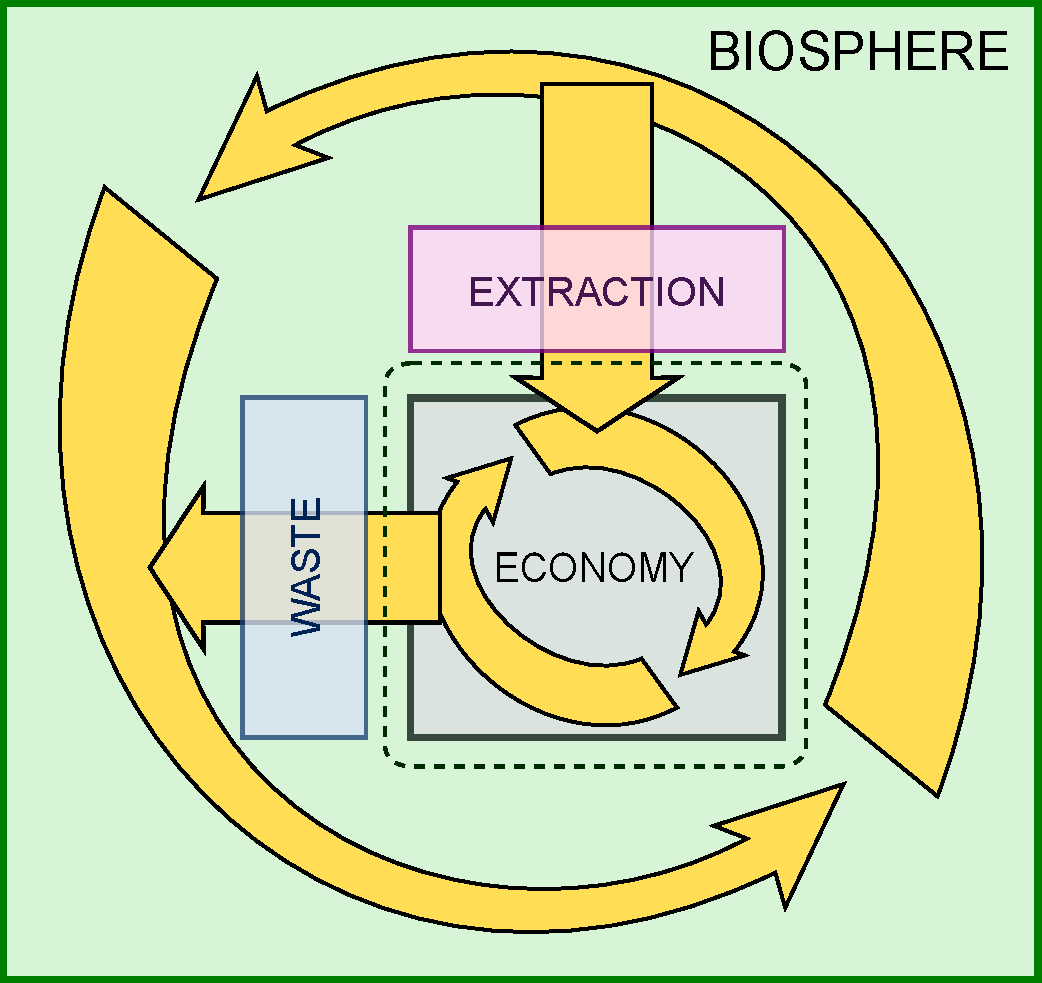
\includegraphics[width=\linewidth]{Part_0/Chapter_Introduction/images/Biosphere_economy_v2.pdf}
\caption[The biosphere and the economy **** MCD - NEED A BETTER FIGURE TITLE ****]
				{The interaction of the economy with the biosphere.
				Materials and energy (yellow arrows) flow around the biosphere.
				Some flows are extracted for human use and enter the economy.
				The materials and energy flow around the economy 
				(as well as accumulating in capital stocks)
				before being emitted as wastes back into the biosphere.
				The size of the arrows does not indicate magnitude of flows.}
\label{fig:biosphere_economy}
\end{figure}


%%%%%%%%%% What to count %%%%%%%%%%
\subsection{What to count}
\label{sec:what_to_count}
%%%%%%%%%% 

We believe the key to understanding how energy transformations will unfold
involves specifically understanding how

\begin{itemize}
	\item{materials,}
	\item{energy,}
	\item{embodied energy, and}
	\item{economic value}
\end{itemize}

\noindent{}each flow and accumulate within society's metabolism, the economy.
Of course, each of the above items interacts with the others 
and the biosphere dynamically.
If we can begin to carefully track these items, 
we will be on our way to gathering the information required to 
assist planning for upcoming materials and energy transformations.

A model informed by the metabolism metaphor may allow consumers, producers,
and policy-makers to answer critical questions that are not
answerable today. Example questions include:

\begin{enumerate}
	\item{What might be the optimal scale of an economy in terms of GDP 
			and what are the impacts of an optimally-sized economy on natural capital?}
    \item{How is fossil fuel dependency embedded in the interlocking fabric of the economy?} 
    \item{How will economies that are dependent on coal, oil, 
 			and other forms of non-renewable energy transition 
			to renewable forms of energy?}
	\item{How might an economy be affected as an increasing share of production
			is directed toward replacing 
			degraded ecosystem services?~\cite[p.~221]{kummel2011}​}
\end{enumerate}

To summarize Sections~\ref{sec:apt_metaphor}--\ref{sec:what_to_count}, 
our approach is to:

\begin{svgraybox}
	develop a dynamic model 
	by applying rigorous thermodynamics 
	to materials and energy flows into, among, 
	and out of economic sectors,
	informed by the metabolism metaphor,
	in a manner that is verifiable against 
	the existing (or expanded) 
	national accounts.
\end{svgraybox}

\noindent{}If successful, we will have developed an analysis framework 
that allows us to \emph{account for the environment}.


%%%%%%%%%% Structure %%%%%%%%%%
\section{Structure of the book}
\label{sec:structure}
%%%%%%%%%%

The bulleted list in Section~\ref{sec:what_to_count} 
provides the beginning of the structure for the rest of this book.

Part~\ref{part:matter} addresses flows of physical matter and energy
through the economy.
Chapter~\ref{chap:materials} discusses material flows and accumulation.
Flows of energy are covered in Chapter~\ref{chap:direct_energy}, 
and a rigorous, thermodynamics-based definition of and accounting for 
embodied energy is presented in Chapter~\ref{chap:embodied_energy}.

In Part~\ref{part:values}, we turn to flow and accumulation of 
non-physical entities through the economy. 
Flows and accumulation of economic value are discussed in Chapter~\ref{chap:value}.
In Chapter~\ref{chap:intensity}, we combine the results from 
Chapters~\ref{chap:embodied_energy} and~\ref{chap:value} to
calculate an important indicator of economic activity:
the energy intensity of economic production.

Part~\ref{part:implications} gives context to the framework developed in
Parts~\ref{part:matter}~and~\ref{part:values}.
Chapter~\ref{chap:implications} draws out some of the direct implications
of our framework.
Chapter~\ref{chap:unfinished_business} looks at 
unfinished business: practical, conceptual, and theoretical issues
that arise in the development of this framework.
And, we end with a summary in Chapter~\ref{chap:summary}.

\begin{table}
\caption[Examples used throughout this book]{Examples
used throughout this book.}
\begin{center}
  \begin{tabular}{c @{\hspace{1.5em}} c @{\hspace{1.5em}} c @{\hspace{1.5em}} c @{\hspace{1.5em}} c}
    \toprule
    Example & Sector 0 & Sector 1 & Sector 2 & Sector 3 \\ 
	\midrule
    A & Biosphere	&	Society            & NA         & NA                 \\
    B & Biosphere	&	Final Consumption  & Production & NA                 \\
    C & Biosphere	&	Final Consumption  & Energy     & Goods \& Services  \\
  \bottomrule
  \end{tabular}
\end{center}
\label{tab:examplesABC}
\end{table}
 
Throughout the methodological chapters~(\ref{chap:materials}--\ref{chap:intensity}),
our accounting framework is developed
through a series of increasingly-disaggregated
models of the economy~(Table~\ref{tab:examplesABC}),
and we use the US auto industry 
as a running example for application and discussion.

**** The next two paragraphs are duplicated from 
Section 2.5 (Materials in the US Auto Industry).
We duplicated them here temporarily so that the editors can 
see the purpose of and justification for the auto industry example. ****

The running example of the US auto industry demonstrates that our dynamic model 
can be tied into national accounts.
The US auto industry example shows where data are available 
(e.g., economic value, Chapter~\ref{chap:value}), 
where it is old (e.g., energy intensity, Chapter~\ref{chap:intensity}), 
and where it has never been available 
(e.g., accumulated embodied energy, Chapter~\ref{chap:embodied_energy}).  
The US auto industry is, therefore, 
illustrative of the challenges inherent 
in obtaining data that would feed the model.

The auto industry 
has been used previously
in the literature in both 
process-based~\cite{Berry:1973vo, Sullivan1995, Stodolsky1995, 
							Sullivan1998, McCleese2002, Sullivan2010, Hawkins2012}
and Input-Output~\cite{Bullard:1978vd, MacLean1998, MacLean2003}
analysis methods,
Furthermore, the industry
remains a large portion of many industrialized economies, 
is very resource intensive, 
has obvious links with energy because
its health is sensitive to disruptions in energy supplies, and
the industry also shows evidence of 
post-industrial decline (shrinking profit margins, etc.).

\bibliographystyle{unsrt}
\bibliography{../../Metabolic}


% Always give a unique label
% and use \ref{<label>} for cross-references
% and \cite{<label>} for bibliographic references
% use \sectionmark{}
% to alter or adjust the section heading in the running head
%% Instead of simply listing headings of different levels we recommend to let every heading be followed by at least a short passage of text. Furtheron please use the \LaTeX\ automatism for all your cross-references and citations.

%% Please note that the first line of text that follows a heading is not indented, whereas the first lines of all sequent paragraphs are.

%% Use the standard \verb|equation| environment to typeset your equations, e.g.
%
%% \begin{equation}
%% a \times b = c\;,
%% \end{equation}
%
%% however, for multiline equations we recommend to use the \verb|eqnarray|
%% environment\footnote{In physics texts please activate the class option \texttt{vecphys} to depict your vectors in \textbf{\itshape boldface-italic} type - as is customary for a wide range of physical jects.}.
%% \begin{eqnarray}
%% a \times b = c \nonumber\\
%% \vec{a} \cdot \vec{b}=\vec{c}
%% \label{eq:01}
%% \end{eqnarray}

%% \section{section Heading}
%% \label{sec:2}
%% Instead of simply listing headings of different levels we recommend to let every heading be followed by at least a short passage of text. Furtheron please use the \LaTeX\ automatism for all your cross-references\index{cross-references} and citations\index{citations} as has already been described in Sect.~\ref{sec:2}.

%% \begin{quotation}
%% Please do not use quotation marks when quoting texts! Simply use the \verb|quotation| environment -- it will automatically render Springer's preferred layout.
%% \end{quotation}


%% \section{section Heading}
%% Instead of simply listing headings of different levels we recommend to let every heading be followed by at least a short passage of text. Furtheron please use the \LaTeX\ automatism for all your cross-references and citations as has already been described in Sect.~\ref{sec:2}, see also Fig.~\ref{fig:1}\footnote{If you copy text passages, figures, or tables from other works, you must obtain \textit{permission} from the copyright holder (usually the original publisher). Please enclose the signed permission with the manucript. The sources\index{permission to print} must be acknowledged either in the captions, as footnotes or in a separate section of the book.}

%% Please note that the first line of text that follows a heading is not indented, whereas the first lines of all sequent paragraphs are.

% For figures use
%
%% \begin{figure}[b]
%% \sidecaption
% Use the relevant command for your figure-insertion program
% to insert the figure file.
% For example, with the option graphics use
%% \includegraphics[scale=.65]{figure}
%
% If not, use
%\picplace{5cm}{2cm} % Give the correct figure height and width in cm
%
%% \caption{If the width of the figure is less than 7.8 cm use the \texttt{sidecapion} command to flush the caption on the left side of the page. If the figure is positioned at the top of the page, align the sidecaption with the top of the figure -- to achieve this you simply need to use the optional argument \texttt{[t]} with the \texttt{sidecaption} command}
%% \label{fig:1}       % Give a unique label
%% \end{figure}


%% \paragraph{Paragraph Heading} %
%% Instead of simply listing headings of different levels we recommend to let every heading be followed by at least a short passage of text. Furtheron please use the \LaTeX\ automatism for all your cross-references and citations as has already been described in Sect.~\ref{sec:2}.

%% Please note that the first line of text that follows a heading is not indented, whereas the first lines of all sequent paragraphs are.

%% For typesetting numbered lists we recommend to use the \verb|enumerate| environment -- it will automatically render Springer's preferred layout.

%% \begin{enumerate}
%% \item{Livelihood and survival mobility are oftentimes coutcomes of uneven socioeconomic development.}
%% \begin{enumerate}
%% \item{Livelihood and survival mobility are oftentimes coutcomes of uneven socioeconomic development.}
%% \item{Livelihood and survival mobility are oftentimes coutcomes of uneven socioeconomic development.}
%% \end{enumerate}
%% \item{Livelihood and survival mobility are oftentimes coutcomes of uneven socioeconomic development.}
%% \end{enumerate}


%% \paragraph{paragraph Heading} In order to avoid simply listing headings of different levels we recommend to let every heading be followed by at least a short passage of text. Use the \LaTeX\ automatism for all your cross-references and citations as has already been described in Sect.~\ref{sec:2}, see also Fig.~\ref{fig:2}.

%% Please note that the first line of text that follows a heading is not indented, whereas the first lines of all sequent paragraphs are.

%% For unnumbered list we recommend to use the \verb|itemize| environment -- it will automatically render Springer's preferred layout.

%% \begin{itemize}
%% \item{Livelihood and survival mobility are oftentimes coutcomes of uneven socioeconomic development, cf. Table~\ref{tab:1}.}
%% \begin{itemize}
%% \item{Livelihood and survival mobility are oftentimes coutcomes of uneven socioeconomic development.}
%% \item{Livelihood and survival mobility are oftentimes coutcomes of uneven socioeconomic development.}
%% \end{itemize}
%% \item{Livelihood and survival mobility are oftentimes coutcomes of uneven socioeconomic development.}
%% \end{itemize}

%% \begin{figure}[t]
%% \sidecaption[t]
% Use the relevant command for your figure-insertion program
% to insert the figure file.
% For example, with the option graphics use
%% \includegraphics[scale=.65]{figure}
%
% If not, use
%\picplace{5cm}{2cm} % Give the correct figure height and width in cm
%
%% \caption{Please write your figure caption here}
%% \label{fig:2}       % Give a unique label
%% \end{figure}

%% \runinhead{Run-in Heading Boldface Version} Use the \LaTeX\ automatism for all your cross-references and citations as has already been described in Sect.~\ref{sec:2}.

%% \runinhead{Run-in Heading Italic Version} Use the \LaTeX\ automatism for all your cross-refer\-ences and citations as has already been described in Sect.~\ref{sec:2}\index{paragraph}.
% Use the \index{} command to code your index words
%
% For tables use
%
%% \begin{table}
%% \caption{Please write your table caption here}
%% \label{tab:1}       % Give a unique label
%
% For LaTeX tables use
%
%% \begin{tabular}{p{2cm}p{2.4cm}p{2cm}p{4.9cm}}
%% \hline\noalign{\smallskip}
%% Classes & class & Length & Action Mechanism  \\
%% \noalign{\smallskip}\svhline\noalign{\smallskip}
%% Translation & mRNA$^a$  & 22 (19--25) & Translation repression, mRNA cleavage\\
%% Translation & mRNA cleavage & 21 & mRNA cleavage\\
%% Translation & mRNA  & 21--22 & mRNA cleavage\\
%%Translation & mRNA  & 24--26 & Histone and DNA Modification\\
%%\noalign{\smallskip}\hline\noalign{\smallskip}
%%\end{tabular}
%%$^a$ Table foot note (with superscript)
%%\end{table}
%
%% \section{Section Heading}
%%\label{sec:3}
% Always give a unique label
% and use \ref{<label>} for cross-references
% and \cite{<label>} for bibliographic references
% use \sectionmark{}
% to alter or adjust the section heading in the running head
%% Instead of simply listing headings of different levels we recommend to let every heading be followed by at least a short passage of text. Furtheron please use the \LaTeX\ automatism for all your cross-references and citations as has already been described in Sect.~\ref{sec:2}.

%% Please note that the first line of text that follows a heading is not indented, whereas the first lines of all sequent paragraphs are.

%%If you want to list definitions or the like we recommend to use the Springer-enhanced \verb|description| environment -- it will automatically render Springer's preferred layout.

%%\begin{description}[Type 1]
%%\item[Type 1]{That addresses central themes pertainng to migration, health, and disease. In Sect.~\ref{sec:1}, Wilson discusses the role of human migration in infectious disease distributions and patterns.}
%%\item[Type 2]{That addresses central themes pertainng to migration, health, and disease. In Sect.~\ref{sec:2}, Wilson discusses the role of human migration in infectious disease distributions and patterns.}
%%\end{description}

%%\section{section Heading} %
%% In order to avoid simply listing headings of different levels we recommend to let every heading be followed by at least a short passage of text. Use the \LaTeX\ automatism for all your cross-references and citations citations as has already been described in Sect.~\ref{sec:2}.

%% Please note that the first line of text that follows a heading is not indented, whereas the first lines of all sequent paragraphs are.

%% \begin{svgraybox}
%% If you want to emphasize complete paragraphs of texts we recommend to use the newly defined Springer class option \verb|graybox| and the newly defined environment \verb|svgraybox|. This will produce a 15 percent screened box 'behind' your text.

%% If you want to emphasize complete paragraphs of texts we recommend to use the newly defined Springer class option and environment \verb|svgraybox|. This will produce a 15 percent screened box 'behind' your text.
%% \end{svgraybox}


%% \section{section Heading}
%%Instead of simply listing headings of different levels we recommend to let every heading be followed by at least a short passage of text. Furtheron please use the \LaTeX\ automatism for all your cross-references and citations as has already been described in Sect.~\ref{sec:2}.

%% Please note that the first line of text that follows a heading is not indented, whereas the first lines of all sequent paragraphs are.

%% \begin{theorem}
%% Theorem text goes here.
%% \end{theorem}
%
% or
%
%% \begin{definition}
%% Definition text goes here.
%% \end{definition}

%% \begin{proof}
%\smartqed
%% Proof text goes here.
%% \qed
%% \end{proof}

%%\paragraph{Paragraph Heading} %
%% Instead of simply listing headings of different levels we recommend to let every heading be followed by at least a short passage of text. Furtheron please use the \LaTeX\ automatism for all your cross-references and citations as has already been described in Sect.~\ref{sec:2}.

%% Note that the first line of text that follows a heading is not indented, whereas the first lines of all subsequent paragraphs are.
%
% For built-in environments use
%
%%\begin{theorem}
%%Theorem text goes here.
%%\end{theorem}
%
%%\begin{definition}
%%Definition text goes here.
%%\end{definition}
%
%%\begin{proof}
%%\smartqed
%% Proof text goes here.
%%\qed
%%\end{proof}
%
%% \begin{acknowledgement}
%% If you want to include acknowledgments of assistance and the like at the end of an individual chapter please use the \verb|acknowledgement| environment -- it will automatically render Springer's preferred layout.
%% \end{acknowledgement}
%
%% \section*{Appendix}
%% \addcontentsline{toc}{section}{Appendix}
%
%% When placed at the end of a chapter or contribution (as opposed to at the end of the book), the numbering of tables, figures, and equations in the appendix section continues on from that in the main text. Hence please \textit{do not} use the \verb|appendix| command when writing an appendix at the end of your chapter or contribution. If there is only one the appendix is designated ``Appendix'', or ``Appendix 1'', or ``Appendix 2'', etc. if there is more than one.

%% \begin{equation}
%% a \times b = c
%% \end{equation}
% Problems or Exercises should be sorted chapterwise
%% \section*{Problems}
%% \addcontentsline{toc}{section}{Problems}
%
% Use the following environment.
% Don't forget to label each problem;
% the label is needed for the solutions' environment
%% \begin{prob}
%% \label{prob1}
%% A given problem or Excercise is described here. The
%% problem is described here. The problem is described here.
%% \end{prob}

%% \begin{prob}
%% \label{prob2}
%% \textbf{Problem Heading}\\
%% (a) The first part of the problem is described here.\\
%% (b) The second part of the problem is described here.
%% \end{prob}


